\begin{figure}
  \begin{center}
    \begin{tabular}{c}
    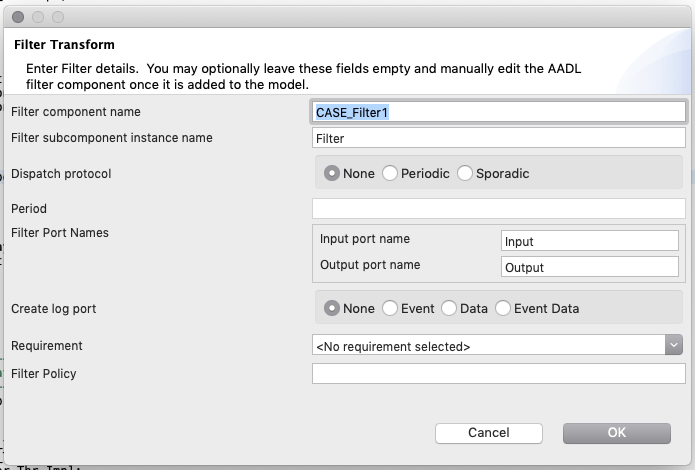
\includegraphics[scale=0.3]{dialogue.png}
    \end{tabular}
  \end{center}
  \caption{BriefCASE dialogue for filter transformation.}
  \label{fig:dialogue}
\end{figure}

\newsavebox{\flt}
\begin{lrbox}{\flt}
  \begin{lstlisting}[style=agree,numbers=left]
    -- start user definitions
    eq policy : bool = 
    WELL_FORMED_AUTOMATION_RESPONSE(Input);
    -- stop user definitions

    guarantee Filter_Output
    "Filter output is well-formed" :
    if event(Input) and policy then 
        event(Output) and Output = Input
    else not event(Output);
  \end{lstlisting}
\end{lrbox}

\newsavebox{\mntr}
\begin{lrbox}{\mntr}
  \begin{lstlisting}[style=agree,numbers=left]
    const is_latched : bool = true;

    -- start user definitions
    const MAX_LATENCY : int = 1;
        
    eq rsp : bool = event(Response);
    eq req : bool = event(Request);

    eq isPending : bool = Since(not rsp, req and not rsp);
    eq latency : int = 0 -> (if req then 0 else pre(latency) + 1);
    
    eq policy : bool = (rsp => req) ->
                        (    (isPending => latency < MAX_LATENCY)   
                        and (rsp => (req or pre(isPending))));
    -- stop user definitions
    
    eq alert : bool = (not policy) -> 
                    ((is_latched and pre(alert)) or not policy);

    assume "One outstanding request at a time" :
    (true -> (req => not pre(isPending))); 
                            
    guarantee "Alert port tracks alert variable" :
    event(Alert) = alert;
    guarantee "Output if not alerted" :
    if (not(alert) and rsp) then
        event(Output) and (Output = Response)
    else
        not (event(Output));    
  \end{lstlisting}
\end{lrbox}

\begin{figure}
  \begin{center}
    \begin{tabular}{c}
      \scalebox{0.62}{\usebox{\flt}} \\
    \end{tabular}
  \end{center}
  \caption{Contract specification for high-assurance filter.}
  \label{fig:filter}
\end{figure}

\begin{figure}
  \begin{center}
    \begin{tabular}{c}
    \scalebox{0.62}{\usebox{\mntr}} \\
    \end{tabular}
  \end{center}
  \caption{Contract specification for high-assurance monitor.}
  \label{fig:monitor}
\end{figure}

As noted previously, the system with the untrusted AI does not pass AGREE verification.
Transformations in BriefCASE are used to cyber-harden the system against malicious AI behavior by inserting a high-assurance filter and monitor between the AI and the WM as shown in \figref{fig:hardened}.
High-assurance means the behaviors of the components are verified.
Here the filter protects the WM from malformed data and the monitor to protects it from spontaneous or delayed responses.
These high-assurance components are added one at a time by selecting the connection in the model where the component is to appear, and then choosing the appropriate transformation.

The system designer provides configuration parameters for the transformation in a dialogue box as shown in \figref{fig:dialogue} for the filter.
All high-assurance components rely on a \emph{policy} to define behavior as seen in the last field of the dialogue box.
A filter policy defines well-formed data while a monitor policy defines an invariant over inputs and outputs.
These policies can be stated directly in the wizard, or they can be left blank and added later to the AGREE contract generated by the transformation.

The BriefCASE creates all the needed AADL for the new high-assurance component and its connections in the system implementation as part of the transformation.
It also creates default AGREE specification that define everything about the component behavior but the policy itself unless it is stated in the dialogue.
The resulting AGREE specification from the transformation for the filter is shown in \figref{fig:filter}.
Here the policy \texttt{WELL\_FORMED\_AUTOMATION\_RESPONSE(Input)} was specified in the dialogue box.
The single guarantee completely defines the filter output under any input according to the truth value of the policy.
While such a string guarantee is not required for AGREE analysis, it is required for automated synthesis.

The resulting AGREE specification for the monitor is shown in \figref{fig:monitor} and is considerable more complex than the filter.

The \texttt{is\_latched} value makes the alert persistent, meaning that once the alert is raised, it is always raised.
This behavior is one of the several options available in the dialogue.
The definition for \texttt{policy} is taken by the system developer from the contract in \figref{fig:sw}.
As before, the guarantees for the outputs are autogenerated by the tool and completely define each output under every possible input.
